% vim:set spell:
% vim:spell spelllang=fr:
\documentclass[a4paper]{article}
\usepackage[utf8x]{inputenc}
\usepackage[T1]{fontenc}
\usepackage{charter}
\usepackage{helvet}
\usepackage{graphicx}
\usepackage{amsmath,amssymb}
\usepackage[french]{babel}
\usepackage{xspace}
\usepackage{setspace}
\setstretch{1.0}
\usepackage{subfigure}
\usepackage{listings}
\voffset       -1in
\hoffset       -1in
\headheight     12pt
\headsep        12pt
\topmargin      25mm
\oddsidemargin  20mm
\textwidth      170mm
\textheight     240mm
\flushbottom
\lstset{numbers=left, numberstyle=\tiny, stepnumber=1, numbersep=5pt}
\graphicspath{{../figures-1-bit/} {../figures-2-bits/} {../figures-simple-global}}
\begin{document}
\begin{center}
\large
Travaux Pratiques Archi SLE-3A\\
\LARGE
Prédiction de branchements\\
\large

\end{center}
\section{Identification}
Travail réalisé par Robin Moussu et Yassine El Khadiri

\section{Prédicteur 1-bit : conception et résultats}
\subsection{code}
Le prédicteur 1 bit est constitué d'un unique tableau de booleens.
Son code est donné ci-dessous.
\small
\begin{verbatim}
// Prédicteur naïf 1-bit qui recopie la dernière décision prise
// Ajout d'une information à la class branch_update à titre d'exemple
class my_update : public branch_update {
public:
        unsigned int index;
};

class my_predictor : public branch_predictor {
   public:
      my_update u;
      branch_info bi;
      // 2^TABLE_BITS entrées de 2 bits
      // TABLE_BITS est passé sur la ligne de commande du compilateur
      unsigned char tab[1<<TABLE_BITS];

      // Constructeur
      my_predictor (void) { 
         memset (tab, 0, sizeof (tab));
      }

      // Calcul de la prédiction
      branch_update *predict (branch_info & b) {
      bi = b;
      if (b.br_flags & BR_CONDITIONAL) {
         // Saut conditionnel
         // Récupération des bits de l'adresse pour indexer la table
         u.index = (b.address & ((1<<TABLE_BITS)-1));
         // Choix de la direction (la mise à jour se fait dans update
         u.direction_prediction (tab[u.index]);
      } else {
         // Saut inconditionnel
         u.direction_prediction (true);
      }
      // Adresse prédite, si on sait le faire
      u.target_prediction (0);
      return &u;
   }

   // Mise à jour de la table de prédiction
   void update (branch_update *u, bool taken, unsigned int target) {
   // Saut conditionnel
   // On peut forcer à true ou false pour avoir les extrêmes
      if (bi.br_flags & BR_CONDITIONAL) {
         tab[((my_update*)u)->index] = taken;
      }
   }
};
// vim:se ts=3:
\end{verbatim}
\normalsize

\subsection{Résultats}
Les résultats issus de la simulation sont les suivants.
\par
\begin{minipage}{.48\linewidth}
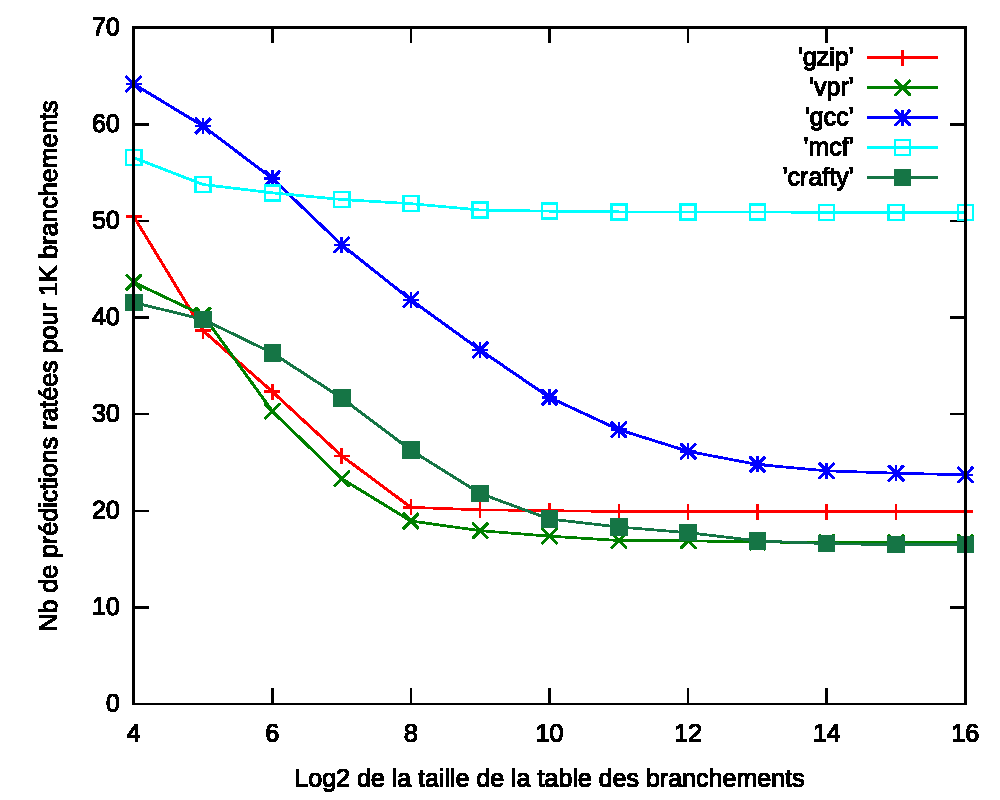
\includegraphics[width=\linewidth]{1-bit-0}
\end{minipage}%
\hfill
\begin{minipage}{.48\linewidth}
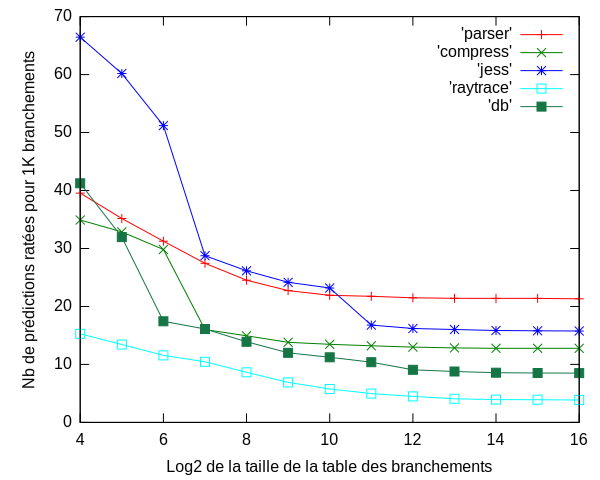
\includegraphics[width=\linewidth]{1-bit-1}
\end{minipage}

\begin{minipage}{.48\linewidth}
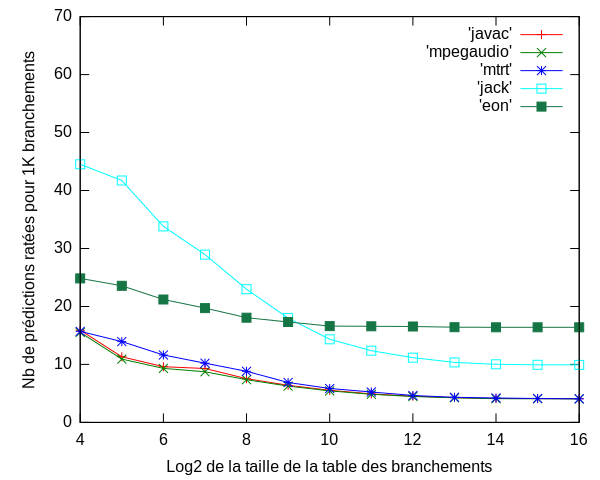
\includegraphics[width=\linewidth]{1-bit-2}
\end{minipage}%
\hfill
\begin{minipage}{.48\linewidth}
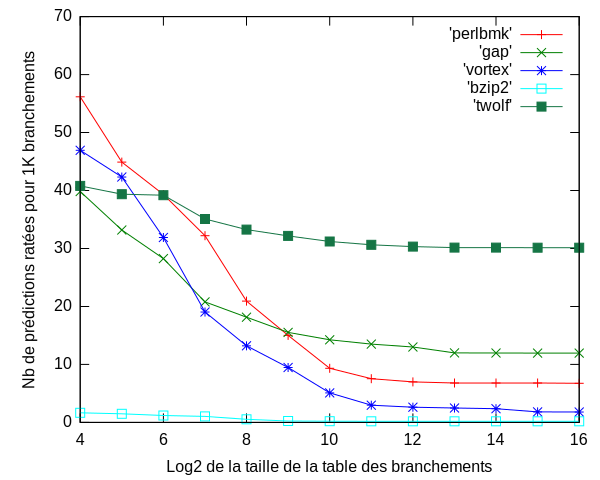
\includegraphics[width=\linewidth]{1-bit-3}
\end{minipage}
\subsection{Analyse}
On voit une asymptote due à la disparition des collisions lorsque la taille du prédicteur augmente.
Le coût du prédicteur est linéaire avec la taille du tableau, et il n'est pas raisonnable de dépasser $2^{16}$ éléments, d'autant que le gain à partir de $2^{12}$ devient très faible.
Par ailleurs, il y a toujours moins de $7\%$ de mauvaise prédictions, ce qui est remarquable pour une approche aussi simpliste.

\section{Prédicteur 2-bits : conception et résultats}
\subsection{code}
Le prédicteur 2 bits est constitué d'un tableau d'états de la machine à état \texttt{ST, T, NT, SNT}.
Son code est donné ci-dessous.
\small
\begin{verbatim}
// Prédicteur 2-bit à 4 états
#ifndef _2_BITS_H
#define _2_BITS_H

#include <vector>

// Ajout d'une information à la class branch_update à titre d'exemple
class my_update : public branch_update {
	 public:
		  unsigned int index;
};

class my_predictor : public branch_predictor {

	 public:

		  enum STATE {
				ST = 0, // 00
				T,  // 01
				NT, // 10
				SNT // 11
		  };
		  // Constructeur
		  // 2^table_bits entrées de STATE
		  my_predictor (unsigned int bits, unsigned int l) :
				table_bits(bits), // Alloue et met à zéro la table
				table(1<<bits, SNT)
		  {}

		  // Calcul de la prédiction
		  branch_update *predict (branch_info & b) {
				bi = b;
				if (b.br_flags & BR_CONDITIONAL) {
					 // Saut conditionnel
					 // Récupération des bits de l'adresse pour indexer la table
					 u.index = (b.address & ((1<<table_bits)-1));
					 // Choix de la direction (la mise à jour se fait dans update
					 u.direction_prediction (state_out(table[u.index]));
				} else {
					 // Saut inconditionnel, 100% sur que c'est pris !
					 u.direction_prediction (true);
				}
				return &u;
		  }

		  // Mise à jour de la table de prédiction
		  void update (branch_update *u, bool taken) {
				// Saut conditionnel
				// On peut forcer à true ou false pour avoir les extrêmes
				if (bi.br_flags & BR_CONDITIONAL) {
					 int index =  ((my_update*)u)->index;
					 STATE s = table[index];
					 table[index] = state_machine(s, taken);
				}
		  }

	 private:
		  my_update u;
		  branch_info bi;
		  unsigned int table_bits;
		  std::vector<STATE> table;


		  bool state_out(STATE s)
		  {
				if (s == ST || s == T) {
					 return true;
				} else {
					 return false;
				}
		  }

		  STATE state_machine(STATE s, bool taken)
		  {
				switch (s){
					 case ST:
						  if (taken)
								return ST;
						  else
								return T;
					 case T:
						  if (taken)
								return ST;
						  else
								return SNT;
						  break;
					 case NT:
						  if (taken)
								return ST;
						  else
								return SNT;
						  break;
					 case SNT:
						  if (taken)
								return NT;
						  else
								return SNT;
						  break;
					 default:
						  return SNT;
				}
		  }
};

#endif // _2_BITS_H
// vim:se ts=3:
\end{verbatim}
\normalsize

\subsection{Résultats}
Les résultats issus de la simulation sont les suivants.
\par
\begin{minipage}{.48\linewidth}
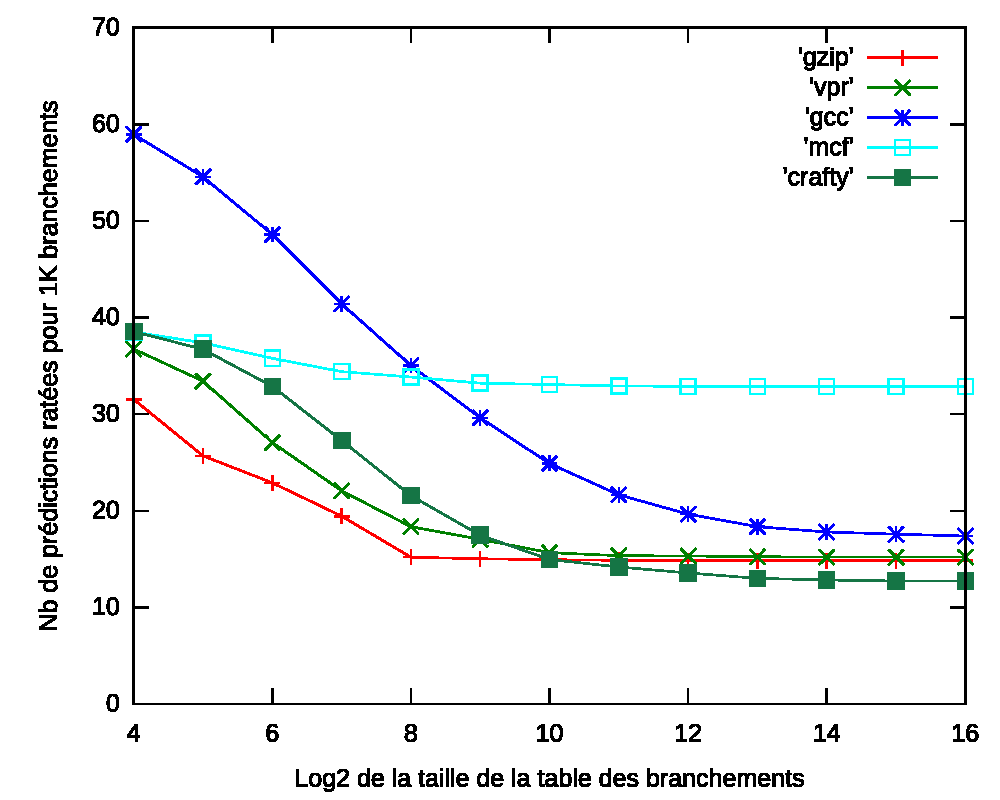
\includegraphics[width=\linewidth]{2-bit-0}
\end{minipage}%
\hfill
\begin{minipage}{.48\linewidth}
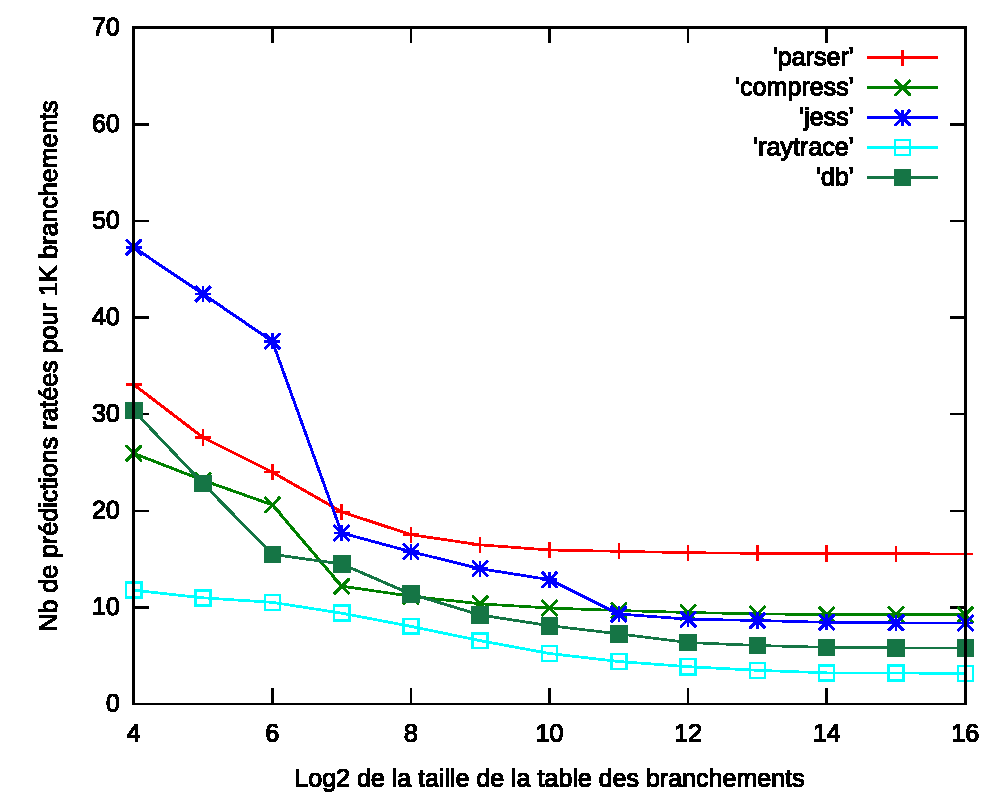
\includegraphics[width=\linewidth]{2-bit-1}
\end{minipage}

\begin{minipage}{.48\linewidth}
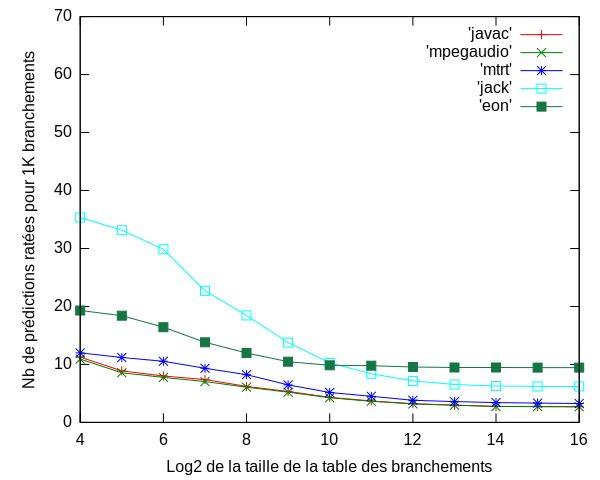
\includegraphics[width=\linewidth]{2-bit-2}
\end{minipage}%
\hfill
\begin{minipage}{.48\linewidth}
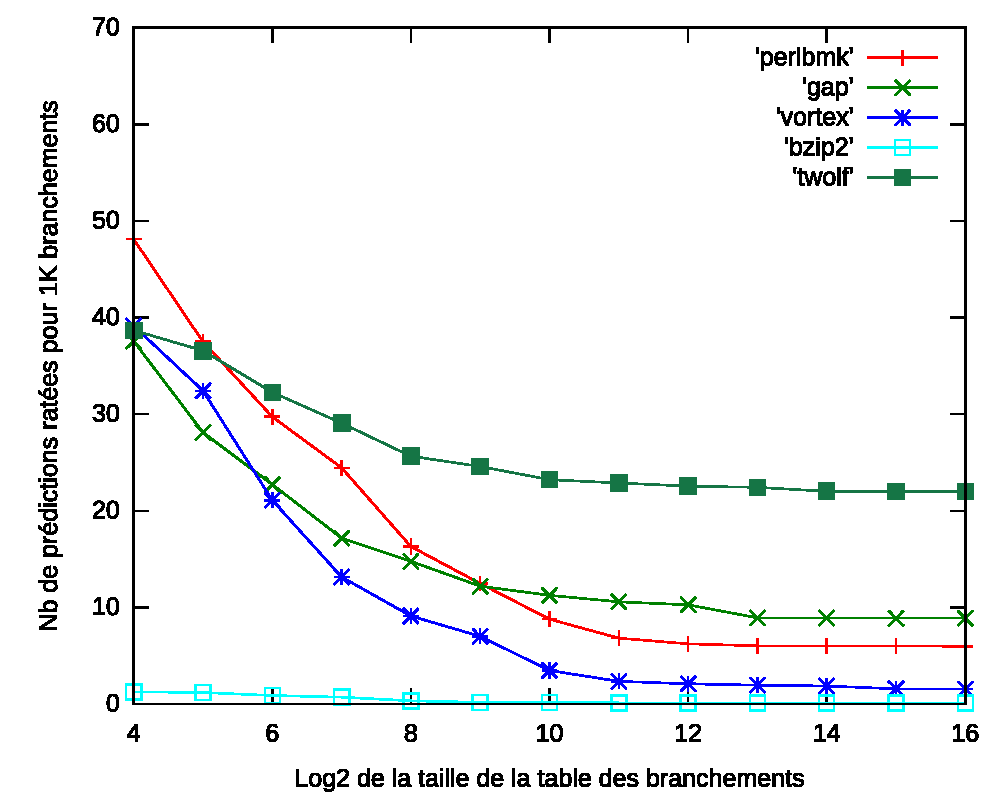
\includegraphics[width=\linewidth]{2-bit-3}
\end{minipage}
\subsection{Analyse}
On remarque une baisse globale considérable du MPKI par rapport aux prédicteur 1-bit dû à la nature hystérésique de la méthode 2-bits.
Par contre la forme des courbes restent la même dû à la similarité des deux méthodes.


\section{Prédicteur global simple : conception et résultats}
\subsection{code}
Le prédicteur global simple est constitué d'un tableau d'états de la machine à état \texttt{ST, T, NT, SNT} indexé par un buffer circulaire.
Son code est donné ci-dessous.
\small
\begin{verbatim}
// Prédicteur simple global à 4 états
#ifndef _2_BITS_H
#define _2_BITS_H

#include <vector>

// Ajout d'une information à la class branch_update à titre d'exemple
class my_update : public branch_update {
	 public:
		  unsigned int index;
};

class my_predictor : public branch_predictor {
	 public:

		  enum STATE {
				ST, // 00
				T,  // 01
				NT, // 10
				SNT // 11
		  };

		  // Constructeur
		  // 2^table_bits entrées de 1 bits
		  my_predictor (unsigned int bits, unsigned int l) :
				table_bits(bits),
				table(1<<bits, SNT),
				mask((1<<l)-1)
		  {
		  }

		  // Calcul de la prédiction
		  branch_update *predict (branch_info & b) {
				bi = b;
				if (b.br_flags & BR_CONDITIONAL) {
					 // Saut conditionnel
					 // Récupération des bits de l'adresse pour indexer la table
					 //u.index = historique.to_int();
					 u.index = hist;
					 // Choix de la direction (la mise à jour se fait dans update
					 u.direction_prediction (state_out(table[u.index]));
				} else {
					 // Saut inconditionnel, 100% sur que c'est pris !
					 u.direction_prediction (true);
				}
				return &u;
		  }

		  // Mise à jour de la table de prédiction
		  void update (branch_update *u, bool taken) {
				// Saut conditionnel
				// On peut forcer à true ou false pour avoir les extrêmes
				if (bi.br_flags & BR_CONDITIONAL) {
					 //int index = historique.to_int();
					 unsigned int index = hist;
					 STATE s = table[index];
					 table[index] = state_machine(s, taken);
					 //historique.push_back(taken);
					 hist = mask & ((hist << 1) | taken);
				}
		  }

	 private:


		  my_update u;
		  branch_info bi;
		  unsigned int table_bits;
		  std::vector<STATE> table;

		  unsigned int hist;
		  // mask pour controller la taille du buffer
		  unsigned int mask;

		  bool state_out(STATE s)
		  {
				if (s == ST || s == T) {
					 return true;
				} else {
					 return false;
				}
		  }

		  STATE state_machine(STATE s, bool taken)
		  {
				switch (s){
					 case ST:
						  if (taken)
								return ST;
						  else
								return T;
					 case T:
						  if (taken)
								return ST;
						  else
								return SNT;
						  break;
					 case NT:
						  if (taken)
								return ST;
						  else
								return SNT;
						  break;
					 case SNT:
						  if (taken)
								return NT;
						  else
								return SNT;
						  break;
					 default:
						  return SNT;
				}
		  }
};

#endif // _2_BITS_H
// vim:se ts=3:
\end{verbatim}
\normalsize

\subsection{Résultats}
Les résultats issus de la simulation sont les suivants.
\par
\begin{minipage}{.48\linewidth}
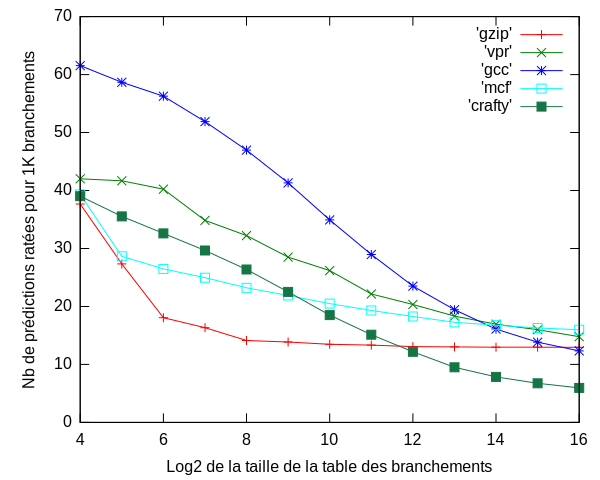
\includegraphics[width=\linewidth]{../figures-simple-global/simple-global-0}
\end{minipage}%
\hfill
\begin{minipage}{.48\linewidth}
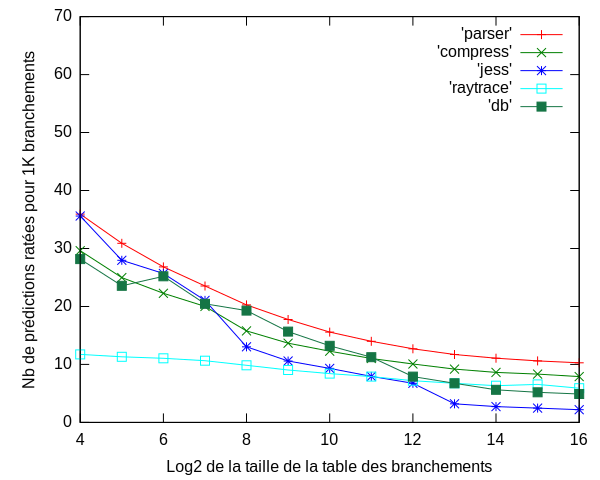
\includegraphics[width=\linewidth]{../figures-simple-global/simple-global-1}
\end{minipage}

\begin{minipage}{.48\linewidth}
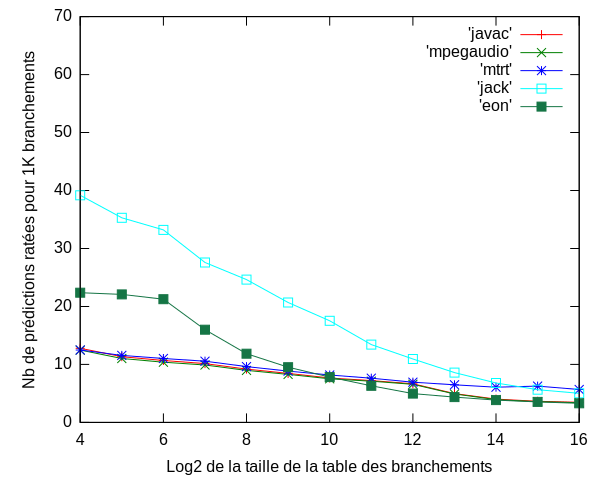
\includegraphics[width=\linewidth]{../figures-simple-global/simple-global-2}
\end{minipage}%
\hfill
\begin{minipage}{.48\linewidth}
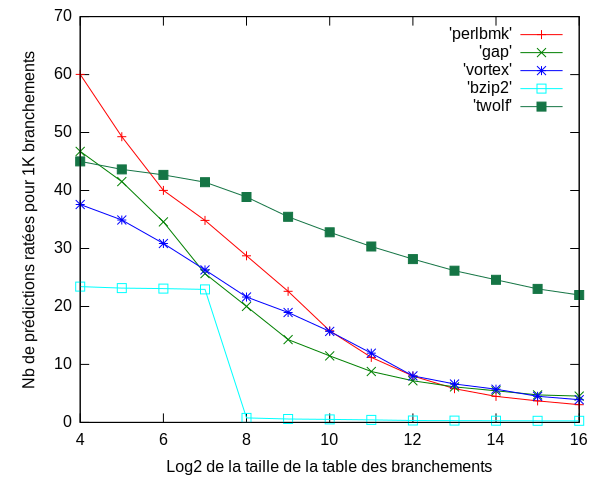
\includegraphics[width=\linewidth]{../figures-simple-global/simple-global-3}
\end{minipage}
\subsection{Analyse}
Le prédicteur simple global ressemble au 2 bits car c'est le même principe avec une méthode d'indexation différente.

\section{Prédicteur gshare : conception et résultats}
\subsection{code}
Le prédicteur gshare est constitué d'un tableau d'états de la machine à état \texttt{ST, T, NT, SNT} indexé par la combinaison d'un buffer circulaire de l'historique des branchements et d'une partie du PC.
Son code est donné ci-dessous.
\small
\begin{verbatim}
// Prédicteur gshare à 4 états
#ifndef _2_BITS_H
#define _2_BITS_H

#include <vector>

// Ajout d'une information à la class branch_update à titre d'exemple
class my_update : public branch_update {
	 public:
		  unsigned int index;
};

class my_predictor : public branch_predictor {
	 public:

		  enum STATE {
				ST, // 00
				T,  // 01
				NT, // 10
				SNT // 11
		  };

		  // Constructeur
		  // 2^table_bits entrées de 1 bits
		  my_predictor (unsigned int bits, unsigned int l) :
				table_bits(bits),
				table(1<<bits, SNT),
				mask((1 << l) - 1)
		  {
		  }

		  // Calcul de la prédiction
		  branch_update *predict (branch_info & b) {
				bi = b;
				if (b.br_flags & BR_CONDITIONAL) {
					 // Saut conditionnel
					 // Récupération des bits de l'adresse pour indexer la table
					 u.index = (b.address & ((1<<table_bits)-1)) xor hist;
					 // Choix de la direction (la mise à jour se fait dans update
					 u.direction_prediction (state_out(table[u.index]));
				} else {
					 // Saut inconditionnel, 100% sur que c'est pris !
					 u.direction_prediction (true);
				}
				return &u;
		  }

		  // Mise à jour de la table de prédiction
		  void update (branch_update *u, bool taken) {
				// Saut conditionnel
				// On peut forcer à true ou false pour avoir les extrêmes
				if (bi.br_flags & BR_CONDITIONAL) {
					 int index =  ((my_update*)u)->index;
					 STATE s = table[index];
					 table[index] = state_machine(s, taken);
					 hist = mask & ((hist << 1) | taken);
				}
		  }

	 private:


		  my_update u;
		  branch_info bi;
		  unsigned int table_bits;
		  std::vector<STATE> table;

		  unsigned int hist;
		  unsigned int mask;

		  bool state_out(STATE s)
		  {
				if (s == ST || s == T) {
					 return true;
				} else {
					 return false;
				}
		  }

		  STATE state_machine(STATE s, bool taken)
		  {
				switch (s){
					 case ST:
						  if (taken)
								return ST;
						  else
								return T;
					 case T:
						  if (taken)
								return ST;
						  else
								return SNT;
						  break;
					 case NT:
						  if (taken)
								return ST;
						  else
								return SNT;
						  break;
					 case SNT:
						  if (taken)
								return NT;
						  else
								return SNT;
						  break;
					 default:
						  return SNT;
				}
		  }
};

#endif // _2_BITS_H
// vim:se ts=3:
\end{verbatim}
\normalsize

\subsection{Résultats}
Les résultats issus de la simulation sont les suivants.
\par
\begin{minipage}{.48\linewidth}
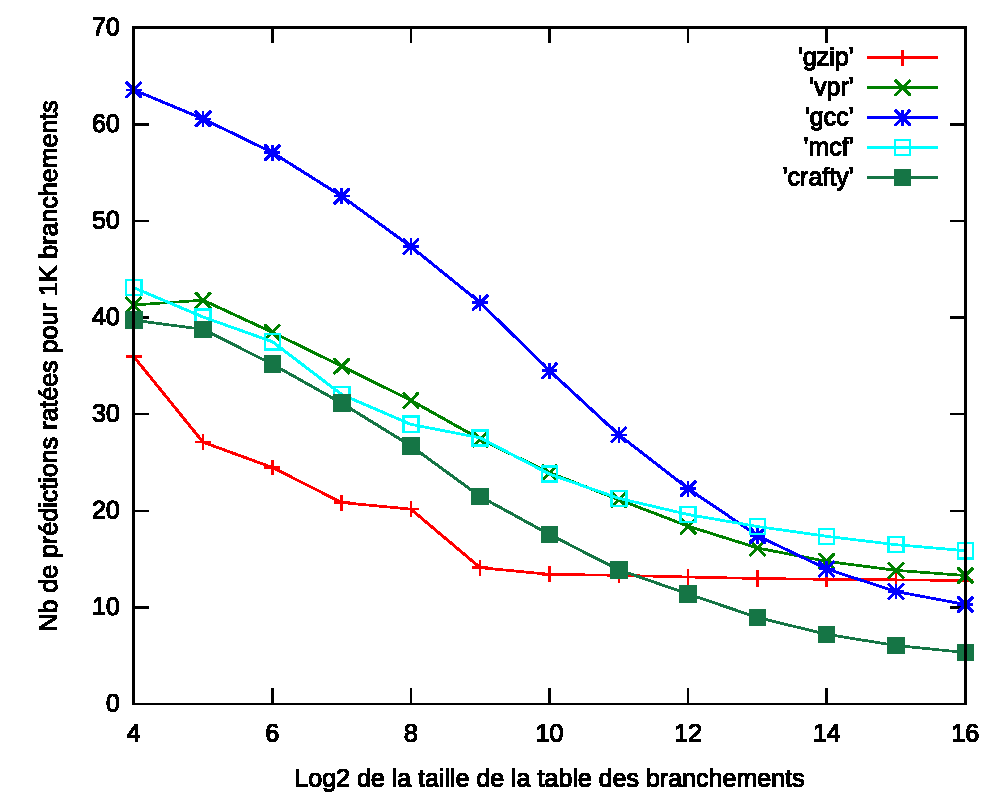
\includegraphics[width=\linewidth]{../figures-gshare/gshare-0}
\end{minipage}%
\hfill
\begin{minipage}{.48\linewidth}
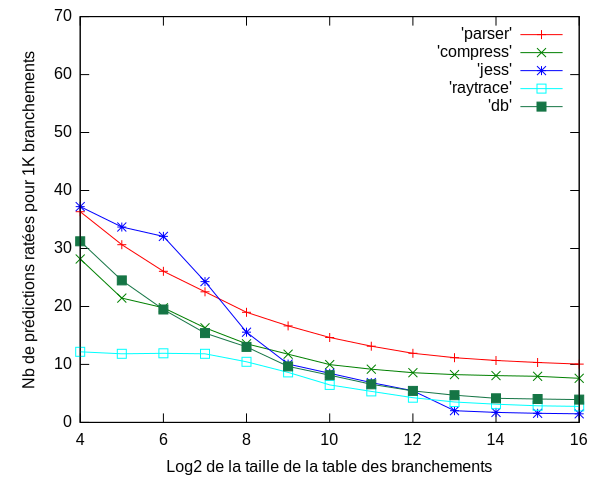
\includegraphics[width=\linewidth]{../figures-gshare/gshare-1}
\end{minipage}

\begin{minipage}{.48\linewidth}
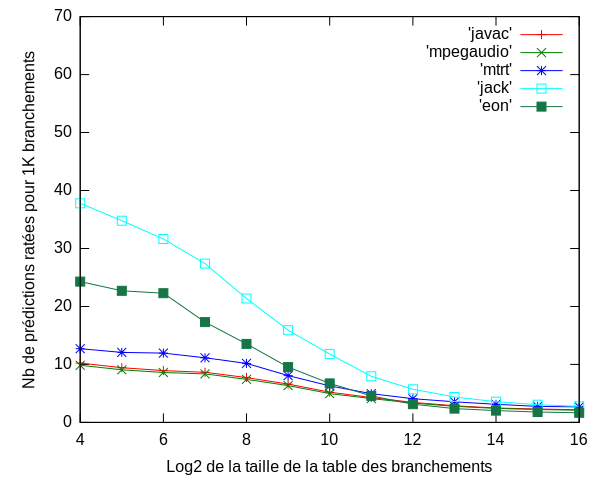
\includegraphics[width=\linewidth]{../figures-gshare/gshare-2}
\end{minipage}%
\hfill
\begin{minipage}{.48\linewidth}
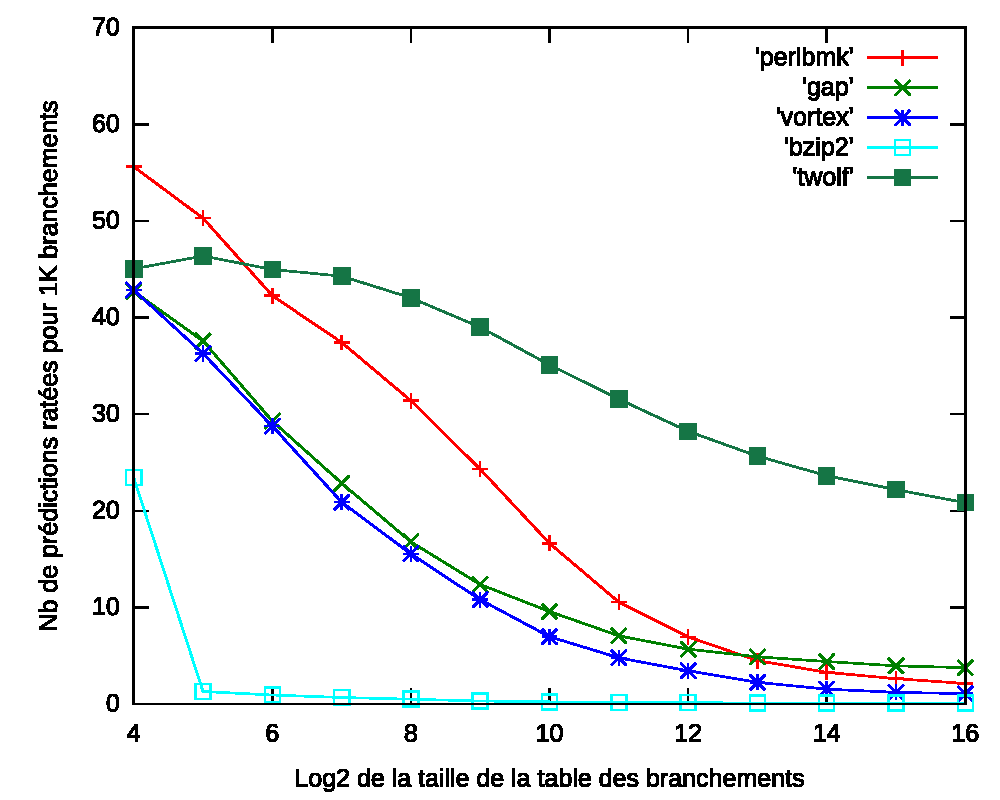
\includegraphics[width=\linewidth]{../figures-gshare/gshare-3}
\end{minipage}
\subsection{Analyse}

\section{Prédicteur corrélé : conception et résultats}
\subsection{code}
Son code est donné ci-dessous.
\small
\begin{verbatim}
// Prédicteur corrélé
#ifndef _CORRELE_H
#define _CORRELE_H

#include <vector>

// Ajout d'une information à la class branch_update à titre d'exemple
class my_update : public branch_update {
	 public:
		  unsigned int index;
};

class my_predictor : public branch_predictor {
	 public:

		  enum STATE {
				ST, // 00
				T,  // 01
				NT, // 10
				SNT // 11
		  };

		  // Constructeur
		  // 2^table_bits entrées de 1 bits
		  my_predictor (unsigned int bits, unsigned int l) :
				table_bits(bits),
				tables(1 << l, std::vector<STATE>(1<<bits, SNT)),
				mask((1 << l) - 1)
		  {
		  }

		  // Calcul de la prédiction
		  branch_update *predict (branch_info & b) {
				bi = b;
				if (b.br_flags & BR_CONDITIONAL) {
					 // Saut conditionnel
					 // Récupération des bits de l'adresse pour indexer la table
					 u.index = (b.address & ((1<<table_bits)-1));
					 // Choix de la direction (la mise à jour se fait dans update
					 u.direction_prediction (state_out(tables[hist][u.index]));
				} else {
					 // Saut inconditionnel, 100% sur que c'est pris !
					 u.direction_prediction (true);
				}
				return &u;
		  }

		  // Mise à jour de la table de prédiction
		  void update (branch_update *u, bool taken) {
				// Saut conditionnel
				// On peut forcer à true ou false pour avoir les extrêmes
				if (bi.br_flags & BR_CONDITIONAL) {
					 int index =  ((my_update*)u)->index;
					 STATE s = tables[hist][index];
					 tables[hist][index] = state_machine(s, taken);
					 hist = mask & ((hist << 1) | taken);
				}
		  }

	 private:

		  my_update u;
		  branch_info bi;
		  unsigned int table_bits;
		  std::vector< std::vector<STATE> > tables;

		  unsigned int hist;
		  unsigned int mask;

		  bool state_out(STATE s)
		  {
				if (s == ST || s == T) {
					 return true;
				} else {
					 return false;
				}
		  }

		  STATE state_machine(STATE s, bool taken)
		  {
				switch (s){
					 case ST:
						  if (taken)
								return ST;
						  else
								return T;
					 case T:
						  if (taken)
								return ST;
						  else
								return SNT;
						  break;
					 case NT:
						  if (taken)
								return ST;
						  else
								return SNT;
						  break;
					 case SNT:
						  if (taken)
								return NT;
						  else
								return SNT;
						  break;
					 default:
						  return SNT;
				}
		  }
};

#endif // _2_BITS_H
// vim:se ts=3:
\end{verbatim}
\normalsize

\subsection{Résultats}
Les résultats issus de la simulation sont les suivants.
\par
\begin{minipage}{.48\linewidth}
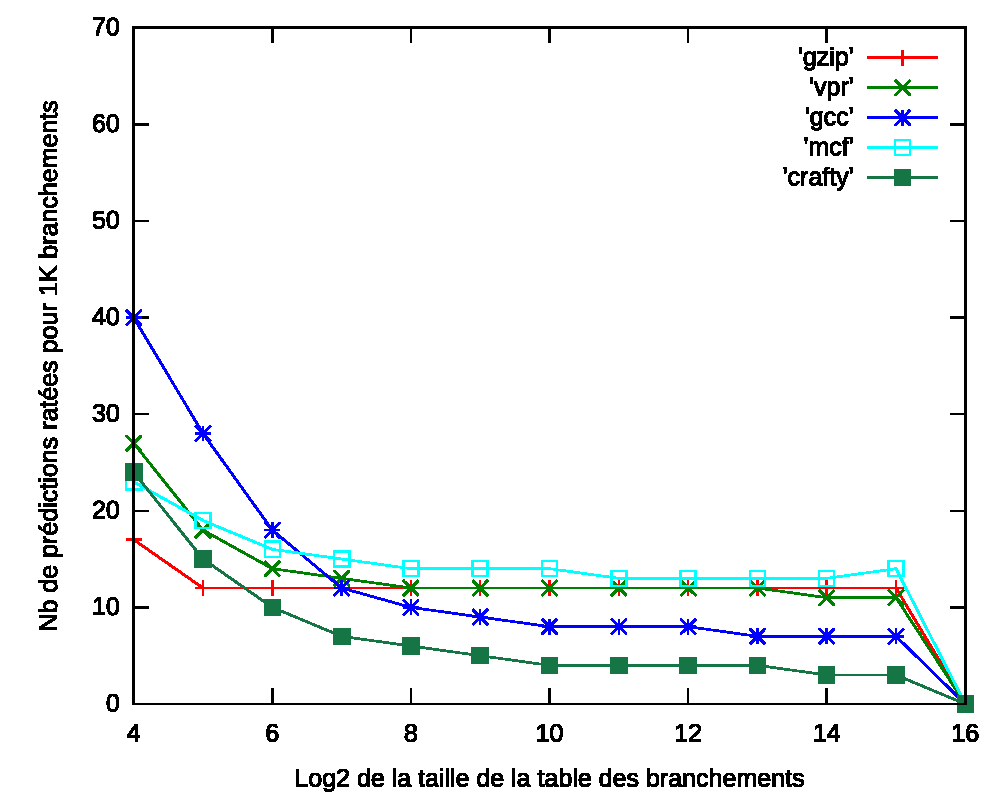
\includegraphics[width=\linewidth]{../figures-correle/correle-0}
\end{minipage}%
\hfill
\begin{minipage}{.48\linewidth}
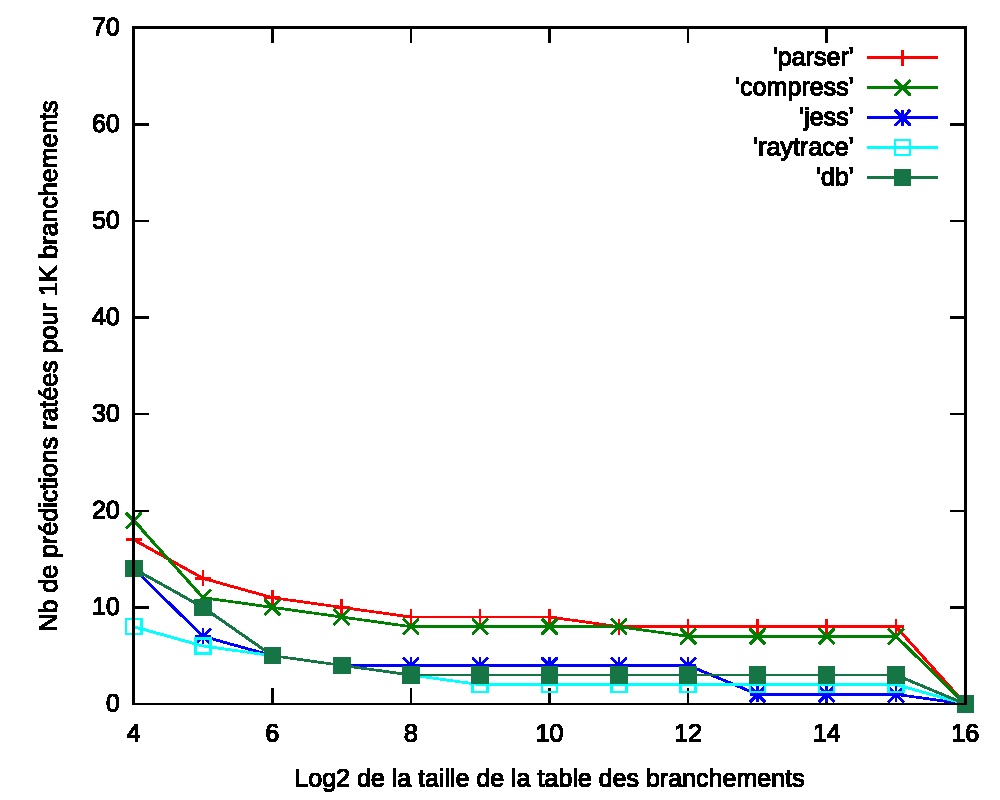
\includegraphics[width=\linewidth]{../figures-correle/correle-1}
\end{minipage}

\begin{minipage}{.48\linewidth}
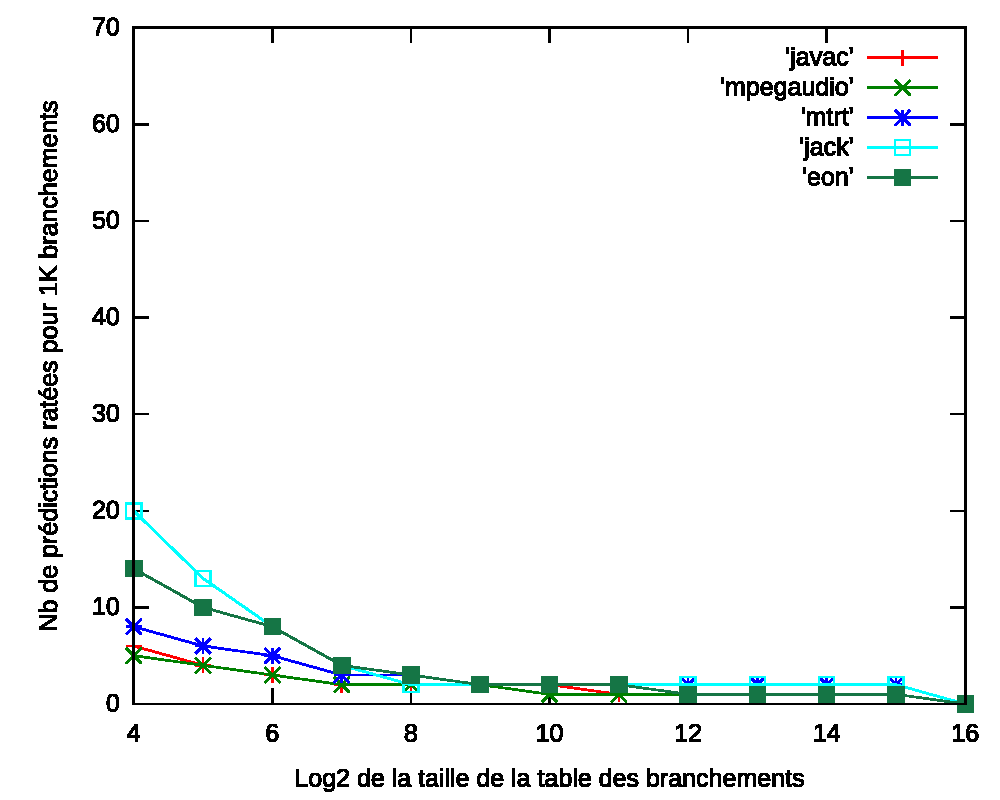
\includegraphics[width=\linewidth]{../figures-correle/correle-2}
\end{minipage}%
\hfill
\begin{minipage}{.48\linewidth}
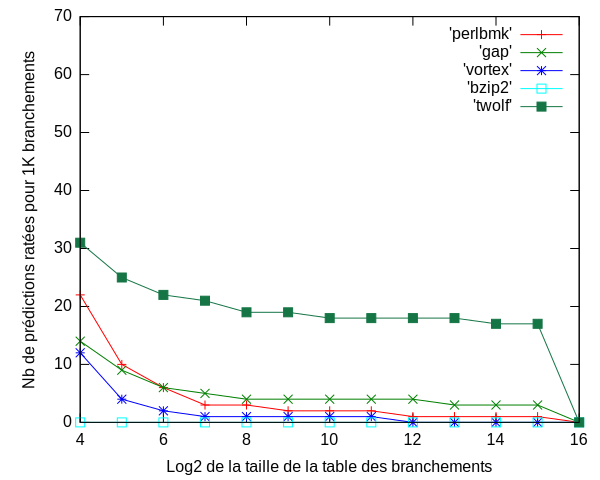
\includegraphics[width=\linewidth]{../figures-correle/correle-3}
\end{minipage}
\subsection{Analyse}

\section{Prédicteur local : conception et résultats}
\subsection{code}
Son code est donné ci-dessous.
\small
\begin{verbatim}
// Prédicteur corrélé
#ifndef _LOCAL_H
#define _LOCAL_H

#include <vector>

// Ajout d'une information à la class branch_update à titre d'exemple
class my_update : public branch_update {
	 public:
		  unsigned int index;
};

class my_predictor : public branch_predictor {
	 public:

		  enum STATE {
				ST, // 00
				T,  // 01
				NT, // 10
				SNT // 11
		  };

		  // Constructeur
		  // 2^table_bits entrées de 1 bits
		  my_predictor (unsigned int bits, unsigned int l) :
				table_bits(bits),
				table(1<<bits, SNT),
				hist(1<<bits, 0),
				mask((1 << l) - 1)
		  {
		  }

		  // Calcul de la prédiction
		  branch_update *predict (branch_info & b) {
				bi = b;
				if (b.br_flags & BR_CONDITIONAL) {
					 // Saut conditionnel
					 // Récupération des bits de l'adresse pour indexer la table
					 u.index = (b.address & ((1<<table_bits)-1));
					 // Choix de la direction (la mise à jour se fait dans update
					 u.direction_prediction (state_out(table[hist[u.index]]));
				} else {
					 // Saut inconditionnel, 100% sur que c'est pris !
					 u.direction_prediction (true);
				}
				return &u;
		  }

		  // Mise à jour de la table de prédiction
		  void update (branch_update *u, bool taken) {
				// Saut conditionnel
				// On peut forcer à true ou false pour avoir les extrêmes
				if (bi.br_flags & BR_CONDITIONAL) {
					 int index =  ((my_update*)u)->index;
					 STATE s = table[hist[index]];
					 table[hist[index]] = state_machine(s, taken);
					 hist[index] = mask & ((hist[index] << 1) | taken);
				}
		  }

	 private:

		  my_update u;
		  branch_info bi;
		  unsigned int table_bits;
		  std::vector<STATE> table;
		  std::vector<unsigned int> hist;
		  unsigned int mask;

		  bool state_out(STATE s)
		  {
				if (s == ST || s == T) {
					 return true;
				} else {
					 return false;
				}
		  }

		  STATE state_machine(STATE s, bool taken)
		  {
				switch (s){
					 case ST:
						  if (taken)
								return ST;
						  else
								return T;
					 case T:
						  if (taken)
								return ST;
						  else
								return SNT;
						  break;
					 case NT:
						  if (taken)
								return ST;
						  else
								return SNT;
						  break;
					 case SNT:
						  if (taken)
								return NT;
						  else
								return SNT;
						  break;
					 default:
						  return SNT;
				}
		  }
};

#endif // _2_BITS_H
// vim:se ts=3:
\end{verbatim}
\normalsize

\subsection{Résultats}
Les résultats issus de la simulation sont les suivants.
\par
\begin{minipage}{.48\linewidth}
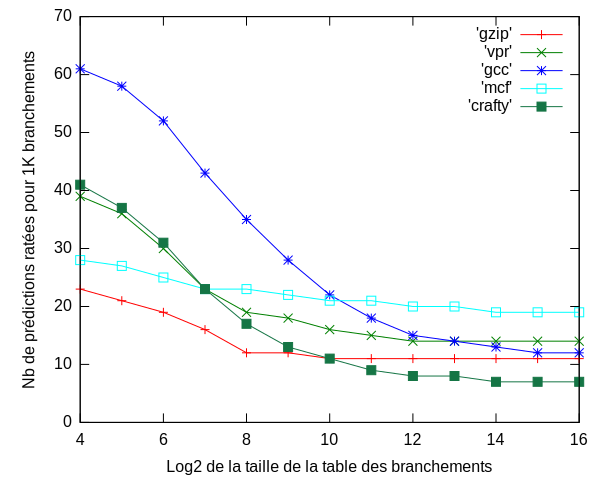
\includegraphics[width=\linewidth]{../figures-local/local-0}
\end{minipage}%
\hfill
\begin{minipage}{.48\linewidth}
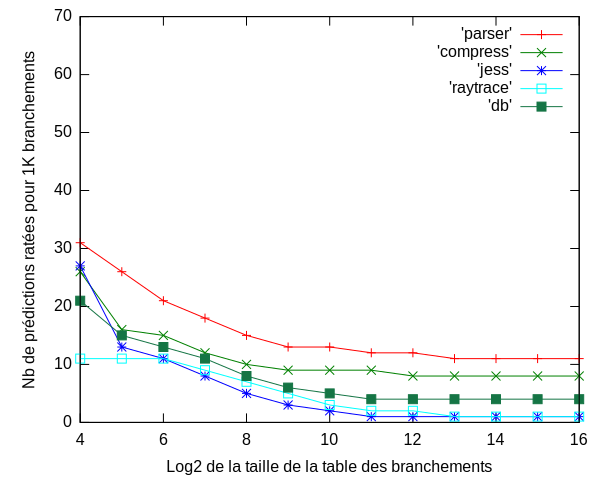
\includegraphics[width=\linewidth]{../figures-local/local-1}
\end{minipage}

\begin{minipage}{.48\linewidth}
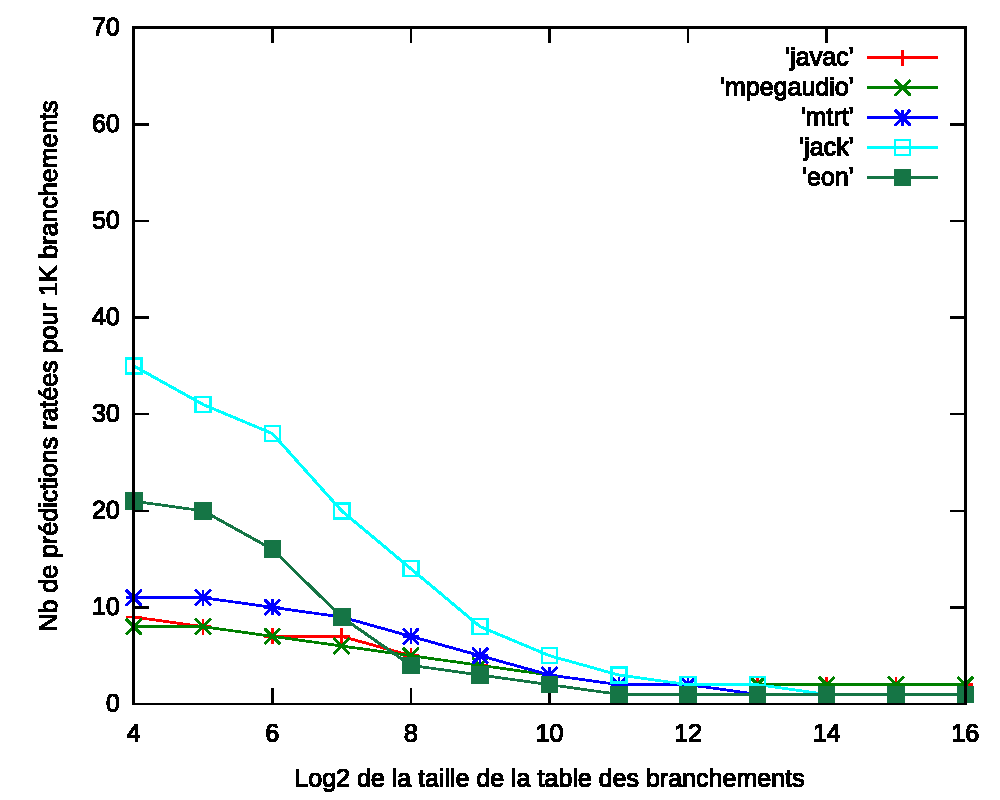
\includegraphics[width=\linewidth]{../figures-local/local-2}
\end{minipage}%
\hfill
\begin{minipage}{.48\linewidth}
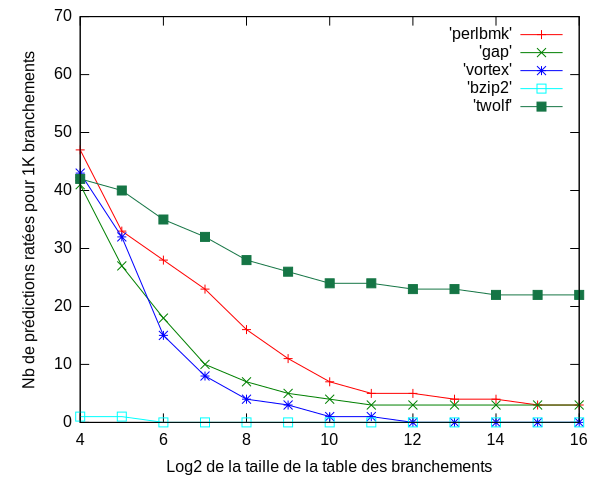
\includegraphics[width=\linewidth]{../figures-local/local-3}
\end{minipage}
\subsection{Analyse}
\end{document}
